\section{Flight tests}
Flight tests were performed to get more practical experience with visual obstacle avoidance.
The system uses a combination of stereo vision and visual odometry for obstacle avoidance, even in GPS-less environments.
These flight tests were performed as part of the \emph{Percevite} project (\url{www.percevite.org}).

\subsection{Stop-before-obstacle with OptiTrack}
\begin{figure}
\centering
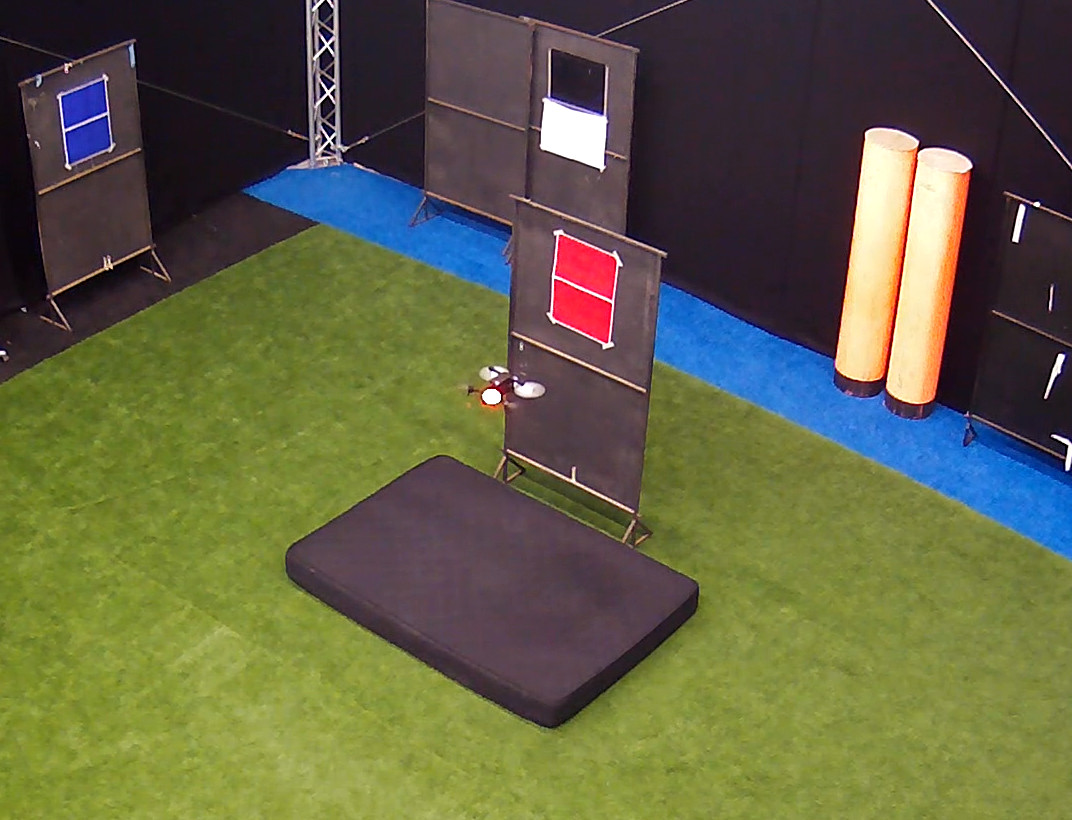
\includegraphics[width=0.75\textwidth]{percevite_optitrack.jpg}
\caption{Parrot Bebop 2 with SLAMDunk stopping in front of an obstacle using \acs{SGBM} and OptiTrack. (March 2018.)}
\label{fig:percevite_optitrack}
\end{figure}



The first task towards obstacle avoidance was the implementation of visual obstacle detection on the Parrot SLAMDunk.
This work started with a review on stereo vision and optical flow (\autoref{sec:sensing}).
The review showed that \acs{SGBM} \cite{Hirschmuller2008} still belongs to the best-performing algorithms.
An implementation of \acs{SGBM} was already present on the SLAMDunk and performed better than the OpenCV implementation due to its use of the GPU.

The depth map obtained from \acs{SGBM} is then used as follows: a \ac{ROI}  is cropped from the center of the image where the view is not occluded by rotors or other parts of the drone.
Of this region, the \nth{5} percentile of depth values is calculated.
The use of the \nth{5} percentile instead of the minimum value adds some robustness to noise, at the cost of missing tiny obstacles (although this has not been a problem in practice).
The \nth{5}-percentile distance is sent to the autopilot as the distance to the nearest obstacle in front of the \ac{UAV}.
Additionally, the number of valid pixels (pixels for which a disparity can be found without ambiguity) is sent to the autopilot; if this value is too low the \ac{UAV} is not allowed to move forward.

The movement logic is implemented as a Paparazzi\footnote{\url{http://wiki.paparazziuav.org/wiki/Main_Page}} autopilot module (but general enough to be ported to other autopilots).
The movement of the \ac{UAV} is controlled using a waypoint; this waypoint can only be moved within the region that is observed to be free of obstacles with a sufficient safety margin.
Since the waypoint is always in a safe region, this should prevent collisions when used in a static environment, provided that the drone can maintain its position without drift.
At this stage, the OptiTrack system inside the TU Delft \cyberzoo\ was used for position feedback, so there was no drift present.

The full system was successfully demonstrated in March 2018 in the \cyberzoo\ (\autoref{fig:percevite_optitrack}).
The code developed for the SLAMDunk/\acs{ROS} is published at \url{https://github.com/tomvand/percevite_slamdunk}, the Paparazzi module is published at \url{https://github.com/tomvand/paparazzi/tree/percevite}.



\subsection{Implementation of `embedded Visual Odometry'}
While the system of March 2018 worked, its dependency on OptiTrack was a strong limitation.
Work on \ac{VO} started with a review of existing methods (\autoref{sec:odo}).
Out of the reviewed methods, the following were evaluated on the SLAMDunk: ORB-SLAM2\footnote{\url{https://github.com/raulmur/ORB_SLAM2}} \cite{Mur-Artal2017}, OKVIS\footnote{\url{https://github.com/ethz-asl/okvis_ros}} \cite{Leutenegger2015} and SVO2\footnote{\url{http://rpg.ifi.uzh.ch/svo2.html}} \cite{Forster2017}.
However, all of these packages had performance issues either in terms of run-time (ORB-SLAM2, OKVIS) or drift (SVO2).
The optical flow algorithm of the Paparazzi autopilot was also evaluated but was found to produce poor velocity estimates or cause segmentation faults, leading to a crash of the autopilot.

Since none of the readily available packages was suitable for use on the SLAMDunk, there was no other choice but to implement a lightweight alternative.
Encouraged by the results of \cite{Marzat2017}, the \emph{\acf{eVO}} algorithm by \citeauthor{Sanfourche2013} \cite{Sanfourche2013} was selected.
The algorithm is a relatively straightforward implementation of \ac{VO} using the \ac{P3P} algorithm.
\ac{P3P} is used to compute the \ac{UAV}'s pose relative to a single keyframe of 3D points; these 3D points are obtained using the depth map of \acs{SGBM}.
The run-time of \ac{eVO} is reduced by using a fixed position for the points in the keyframe; these are not further refined when new measurements arrive.
Secondly, the gyroscope is used to predict the next positions of the keypoints, thereby lowering the search region for the optical flow algorithm.
My implementation of \ac{eVO} is published at \url{https://github.com/tomvand/openevo} (and \url{https://github.com/tomvand/openevo-ros} for the \ac{ROS} wrapper).
This implementation does not reach the run-times reported in \cite{Sanfourche2013}, but still runs at a rate of $\sim 5-\SI{10}{\Hz}$ on the SLAMDunk.

\begin{figure}
\centering
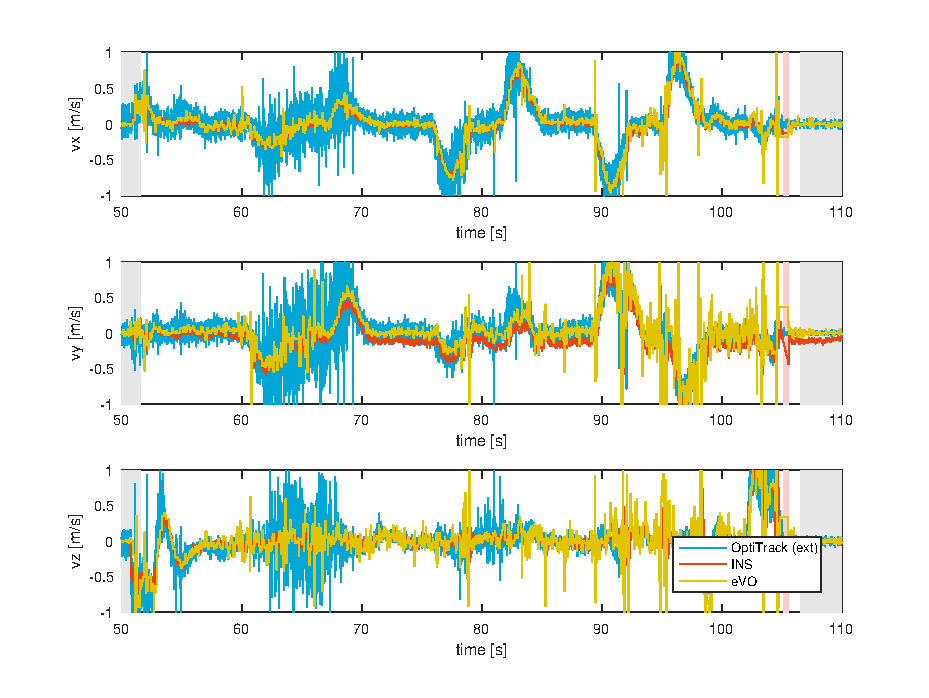
\includegraphics{evo_velocity.pdf}
\caption{Body-frame velocities estimated using \ac{eVO} compared to the ground-truth from OptiTrack. The figure shows both the raw estimates (eVO) and the velocity estimates after fusion with the accelerometer readings (INS). In general the estimate of \ac{eVO} corresponds well to the OptiTrack measurements and appears to be less noisy (this may depend on the OptiTrack calibration and lighting conditions in the \cyberzoo). The INS estimates have a slight bias (especially in the y axis) that comes from the accelerometer. Possibly the SLAMDunk is not placed exactly above the \ac{CoG} of the drone.}
\label{fig:evo_velocity}
\end{figure}

\begin{figure}
\centering
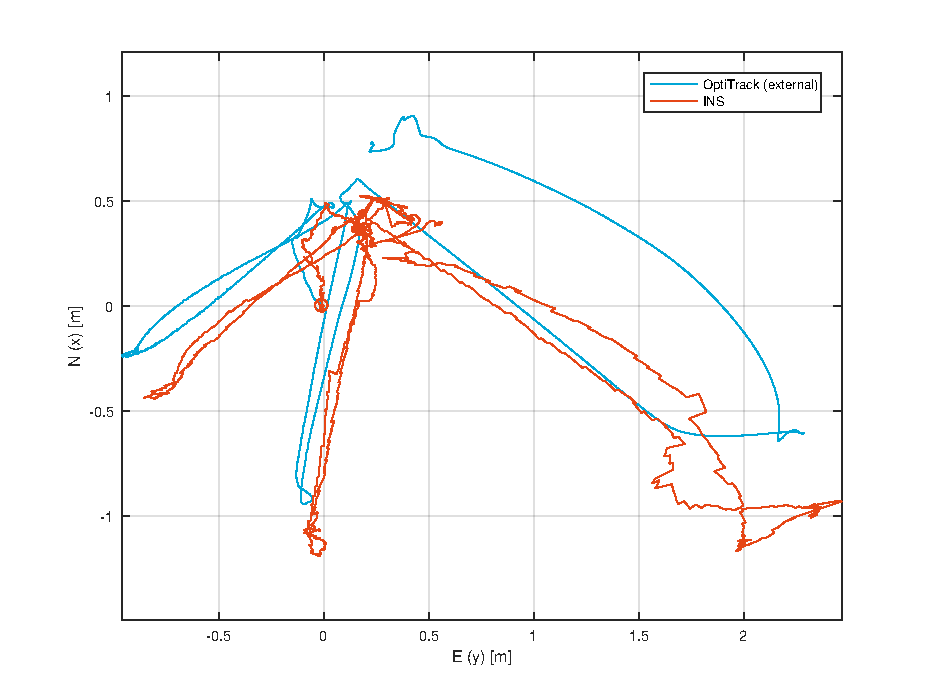
\includegraphics{evo_trajectory.pdf}
\caption{\ac{UAV} trajectory estimated using \ac{eVO} as input to the INS, compared to the ground truth captured using the OptiTrack system. The starting position of the \ac{UAV} is indicated by the circle at $(0,0)$. The final position error was \SI{50}{\centi\meter} after a flight of \SI{60}{\s}.}
\label{fig:evo_trajectory}
\end{figure}

\begin{figure}
\centering
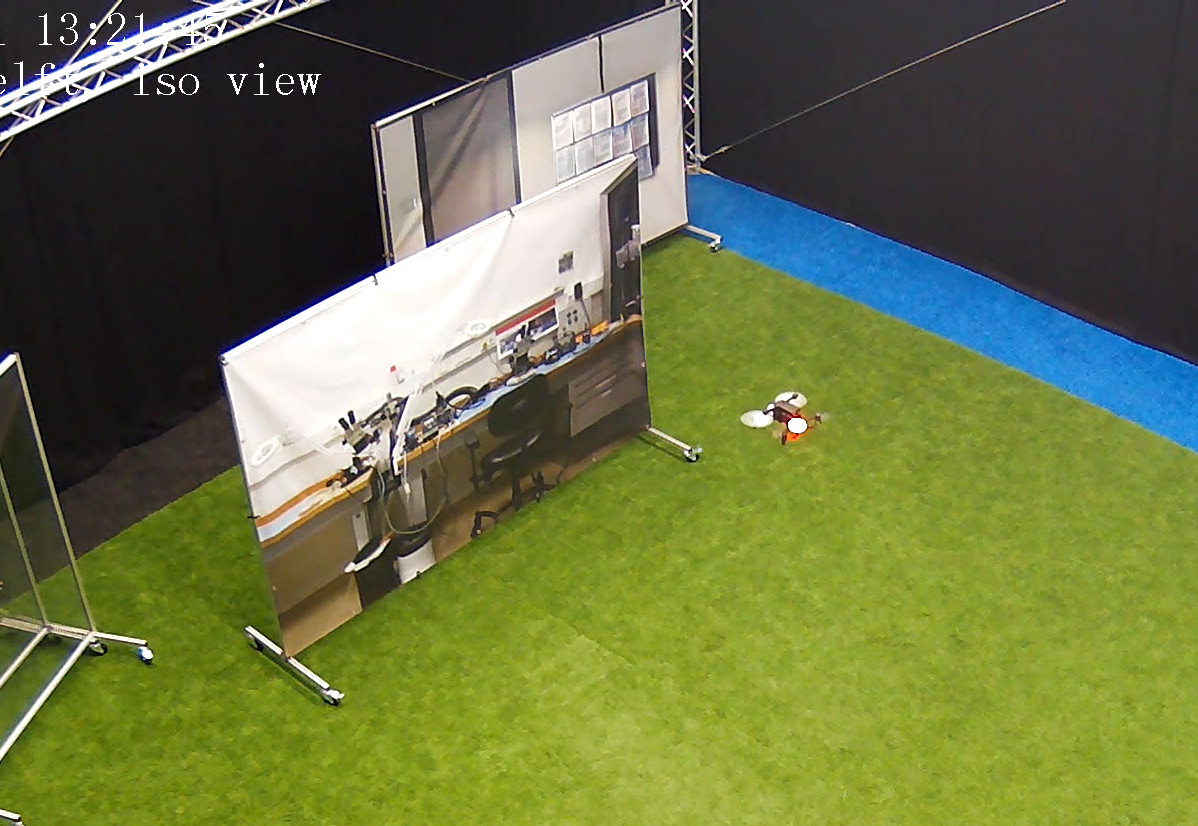
\includegraphics[width=0.75\textwidth]{percevite_evo.jpg}
\caption{Stop-before-obstacle using \ac{eVO}. (July 2018.)}
\label{fig:evo_stop}
\end{figure}

The velocity estimates from \ac{eVO} are sent to Paparazzi, where the horizontal \ac{EKF} combines the velocities with accelerometer measurements to get a final estimate of the \ac{UAV}'s velocity and position.
The world position and angular rates -- also estimated by \ac{eVO} -- are currently unused.
The \ac{eVO} algorithm was tested inside the \cyberzoo\ and found to be surprisingly robust: it was able to follow the drone's trajectory even when no textured panels were placed around the edge of the \cyberzoo.
Test flight results are shown in \autoref{fig:evo_velocity} and \ref{fig:evo_trajectory}.
The drone could successfully navigate between waypoints and stop in front of obstacles (\autoref{fig:evo_stop}).




\subsection{Outdoor test flights}
\begin{figure}
\centering
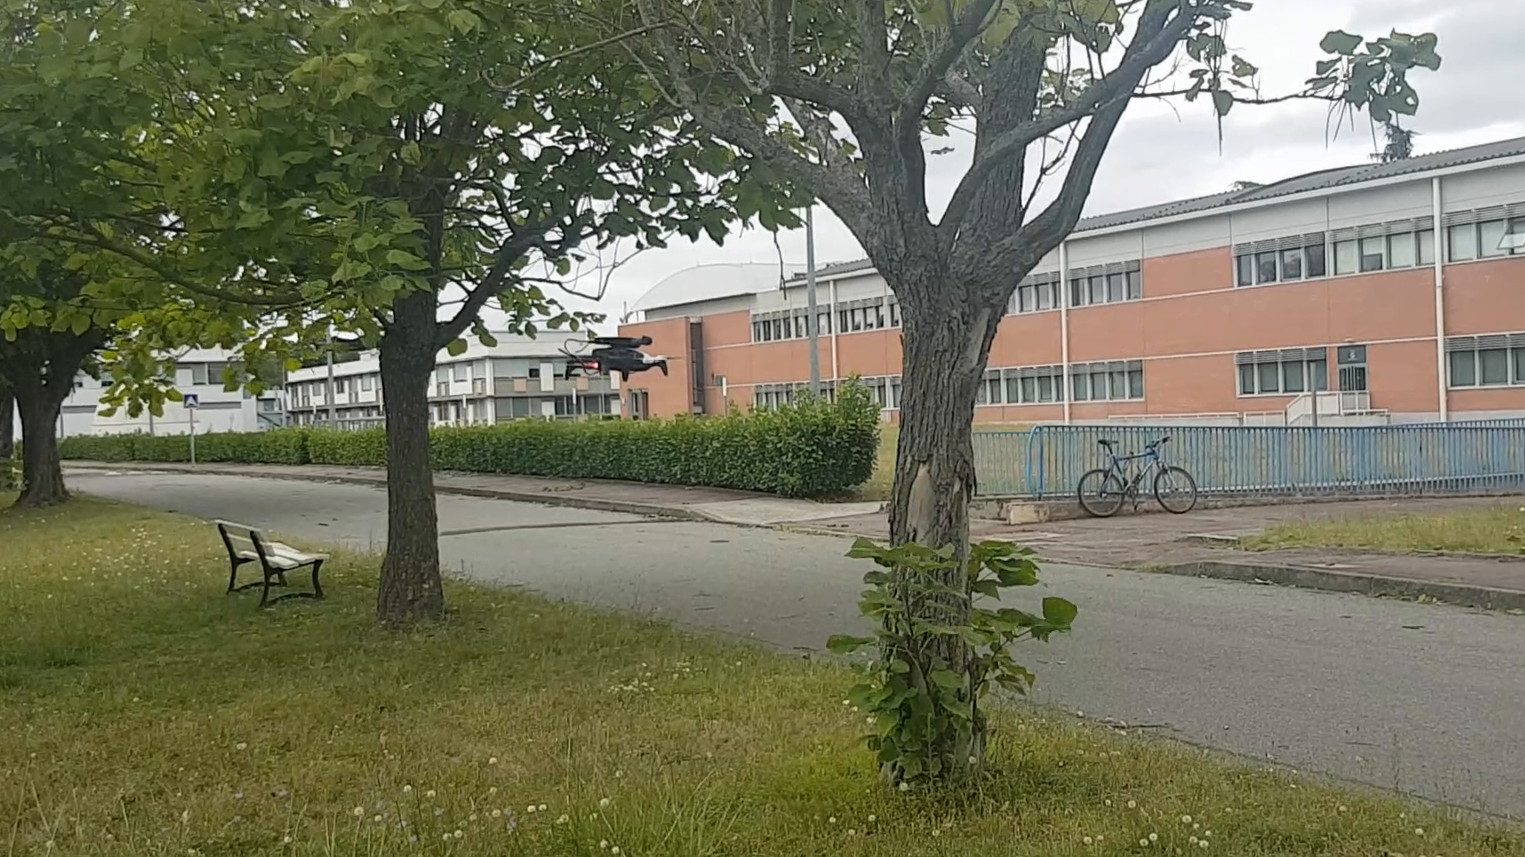
\includegraphics[width=0.45\textwidth]{enac_tree.jpg}
~
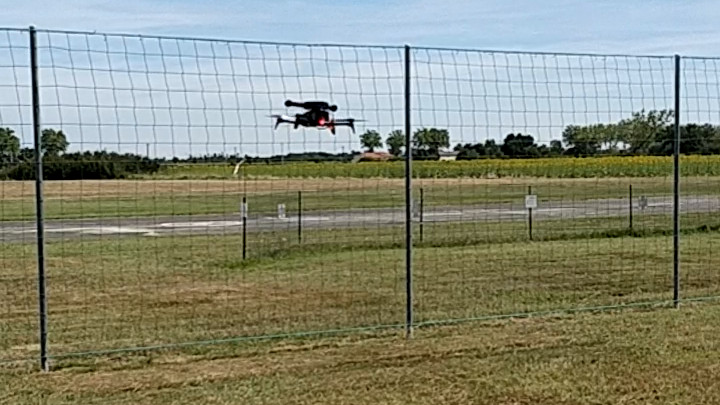
\includegraphics[width=0.45\textwidth]{enac_fence.jpg}
\caption{Outdoor stop-before-obstacle tests at \acs{ENAC}. (August 2018.)}
\label{fig:enac_obstacle}
\end{figure}

Outdoor test flights allowed \ac{eVO} and \acs{SGBM} to be tested in real outdoor environments with natural obstacles and lighting and under windy conditions.
The velocity estimate of \ac{eVO} was found accurate enough for the \ac{UAV} to maintain its position under windy conditions.
\acs{SGBM} was able to reliably detect obstacles, although it produced a few false positive detections when facing the sun.
Tests of the full obstacle avoidance system were performed by sending the drone towards obstacles.
In most of the cases the drone stopped successfully in front of the obstacle (\autoref{fig:enac_obstacle}).

A second goal of the outdoor flights was to add \ac{GPS} to the position estimate of the drone.
The use of \ac{GPS} allows the \ac{UAV} to follow pre-programmed trajectories and is more in line with the target applications.
Fusion of \ac{GPS} with \ac{eVO} velocity estimates was successfully demonstrated during short test flights.
Longer \ac{GPS} trajectories were however not tested because of battery limitations.

During the outdoor tests the ground-truth position of the drone could not be recorded, most test flights are instead recorded as videos of the \ac{UAV} combined with logs of its internal estimates.
The outdoor tests were very successful; during the week the \ac{UAV} only crashed once, possibly as the result of human error instead of an algorithm failure.

\medskip
\noindent
\emph{The collision avoidance system described here was used in the International Micro Air Vehicle (IMAV) competition 2018, where the ENAC/TU DELFT Team Paparazzi reached first place in the outdoor competition. \url{http://www.imavs.org/imav-2018-awards/}}


